\documentclass[titlepage]{article}
\usepackage{array}
\usepackage{enumerate}
\usepackage{graphicx}
\usepackage{listings}

\begin{document}

\author{Stevan Stanisic and Santana Mach}
\title{COMP 8505 - Final Project \\ Rootkit \\ Design Documents}
\date{Nov 06, 2011}
\maketitle{}

\tableofcontents
\pagebreak

\section{Introduction}

Need an intro...

\section{Program Functionality}

\begin{lstlisting}
Pseudo-code for Client Program
\{
	Pseudo code goes here

	...
\}
\end{lstlisting}

\begin{lstlisting}
Pseudo-code for Server Program
\{
	Pseudo code goes here

	...
\}
\end{lstlisting}

\section{Communication Details}

\subsection{State Machine}

\begin{figure}[htb]                                                                       
  \begin{center}
    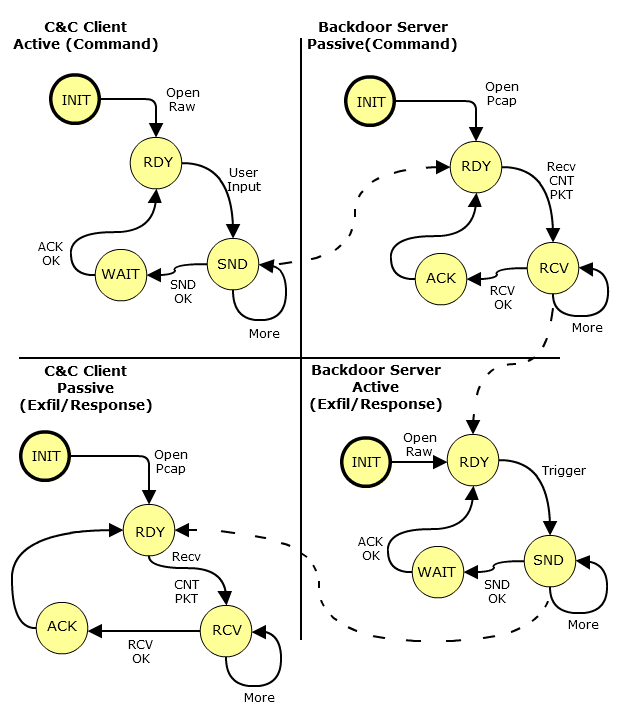
\includegraphics[width=0.9\textwidth]{imgs/std.png}
  \end{center}
  \caption{Program State Transition Diagram}
  \label{fig:std}
\end{figure}

\begin{figure}[htb]                                                                       
  \begin{center}
    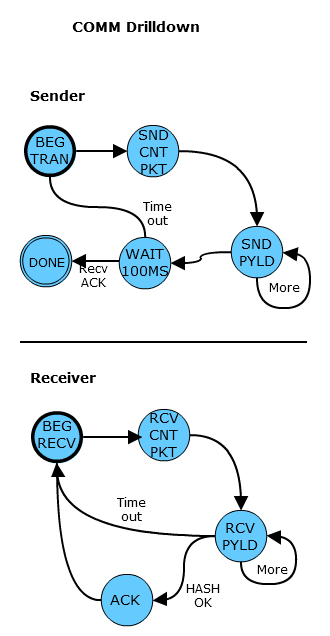
\includegraphics[width=0.5\textwidth]{imgs/comm.png}
  \end{center}
  \caption{Transmission State Transition Diagram}
  \label{fig:comm}
\end{figure}

\begin{lstlisting}
Pseudo-code for State Machine
\{
	Pseudo code goes here

	...
\}
\end{lstlisting}

\subsection{Covert Channel}

\begin{figure}[htb]                                                                       
  \begin{center}
    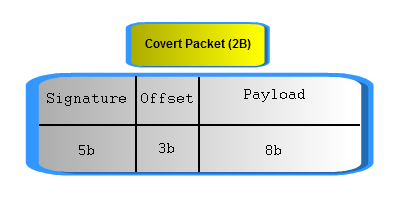
\includegraphics[width=0.9\textwidth]{imgs/packet.png}
  \end{center}
  \caption{Packet Data Diagram}
  \label{fig:packet}
\end{figure}

\begin{figure}[htb]                                                                       
  \begin{center}
    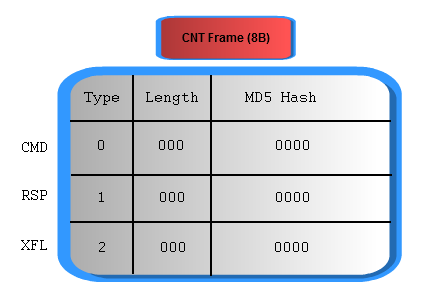
\includegraphics[width=0.9\textwidth]{imgs/frame.png}
  \end{center}
  \caption{Control Frame Diagram}
  \label{fig:frame}
\end{figure}

\begin{figure}[htb]                                                                       
  \begin{center}
    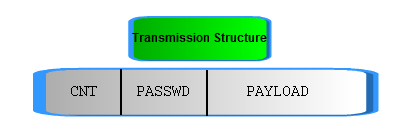
\includegraphics[width=0.9\textwidth]{imgs/transmission.png}
  \end{center}
  \caption{Overall Transmission Diagram}
  \label{fig:transmission}
\end{figure}

\section{Conclusion}

\end{document}
